\section{Model Robustness and Drift Detection}
    In this chapter the stability and robustness of the trained models are presented. First subsection shows models' performance on the corrupted DIC input data with two sources of corrupted signal: artificial pseudocorruptions and real corruptions from the microscope settings. It presents the influence of augmentations on the robusteness, studies the influence of corruptions on practical biological metrics and shows how generalizable the models are across phenotypes. Second subsection presents a study of the image representations in the UNet embeddings including their possible clustering in the lower dimensional space based on several possible clustering hypotheses. And finally the last subsection covers the results of the drift detection algorithm built to alert end users when models predictions become unreliable. Which happends when there is a difference between the data used for training and the data used during inference. 
    \subsection{Stability study}
    For practical reasons it is important to not only evaluate the models on high-quality data exclusively, but also to know how the predictions will degrade when the input's data quality decreases. Having a model for fluorescence \textit{in silico} labeling that can additionally alarm end use when the predictions should not be relied upon is very useful in practice. Although the DIC microscopy is a relatively easy technique, there are still setting up procedures taking place that can be prone to errors. Additionally, as the models are not easily generalizable across phenotypes as well as between fixed and not fixed cells, an alarming system that is able to catch these situations would be useful to save time and cost of lab work. In order to measure the stability or robustness of the models towards data degeneration they were evaluated on the corrupted or "bad" input DIC images. There are two sources of "bad" images that can be used for such estimations. The first are actually corrupted images made in the laboratory. Such corruptions may come from different sources: for example, an oil bubble landed on the microscope lenses, low density of the cell on the image, over- or underexposure during image acquisition. Another source of image corruption would be images with artificial or pseudocorruptions created manually via image processing. 
    
    %This chapter first provides a description of artificial corruptions used to evaluate previously trained models on. Afterwards the real examples of corruptions acquired from the lab are 
    \subsubsection{Artificial corruptions}
        
In this subsection results from evaluating models on three types of artificial image corruption are presented, namely: defocus blur that imitates the defocus of the microscope lenses, changes in brightness and changes in contrast. Every corruption  has different effects on the prediction of the model based on its severity level. Therefore it is important to evaluate the error-rate (in this case a loss function) for the predictions for different severity levels of each corruption type presented. It is also important to perform a visual evaluation of the model's predictions on corrupted data. Each corruption $c$ has severity levels $s$, where $-5 \leq s \leq 5$ ($0 \leq s \leq 5$ for defocus blur corruption). $0$ here corresponds to an original image without corruption. It is important to keep in mind that although severity levels were chosen to be as much comparable between one another as possible, they still might have differences in their strengths. For example, contrast has much stronger effect on predictions than brightness changes. Three types of artificial image corruption are presented below.

\subsubsection{Defocus Blur}
\label{section:defocus-blur}
Defocus blur corruption imitates the effect of defocus on the microscope. The blur is applied to the image by convolving it with a special defocus kernel. There are two tunable parameters for this corruption type: the first one is the radius of the circle in the kernel $r$, and the second one is the blur strength parameter $s$. An example of the kernel with radius $r$ is shown in the Figure \ref{fig:defocus-blur-kernel}. This kernel is then simply applied to an image via $cv2.filter2D$ function.

\begin{figure}[htb]
	\begin{center}
		
\includegraphics[width=0.2\linewidth]{bilder/stability/defocus-blur-kernel.png}
		\caption{Defocus blur kernel}\label{fig:defocus-blur-kernel}
	\end{center}
\end{figure}

\subsubsection{Brightness}
Different brightness levels are also an important image corruption to perform tests on. Brightness variations appear often in the dataset during image acquisition. In order to change the brightness, an image from the RGB format was translated into HSV format, which stands for hue, saturation and value. This is also one of the popular formats to represent an image. To make an image brighter or darker, one can simply add or subtract a parameter $s$ in a value channel for each pixel $x_{i,j}$ correspondingly. This parameter is often called bias. The bigger absolute value of this of this change, the stronger a corruption will occur.

\begin{equation}
    \hat{x}_{i, j} = x_{i, j} + s
\end{equation}

\subsubsection{Contrast}
In contrast to adding a constant value pixelwise to an image in order to change a contrast level, one can perform a multiplication of an image with another constant $s$. This parameter is often called gain.

\begin{equation}
    \hat{x}_{i, j} = s * x_{i, j}
\end{equation}

For both contrast and brightness changes one can use $cv2.convertScaleAbs()$ from the OpenCV library. This method directly accepts gain and bias parameters and clips the image to stay within the allowed range of values.

The values of hyperparameters used in corruptions (kernel radius, gain and bias) are stretched across the range of severity levels and presented in Table \ref{table:corruption-hyperparameters}.
\begin{table}[htb]
    \centering
    \caption{Hyperparameterization for different artificial corruption severities}
        \begin{adjustbox}{width=1\textwidth}
            \begin{tabular}{|l||*{11}{c|}}\hline
                \backslashbox{Corruption}{Severity}
                &\makebox[3em]{-5}
                &\makebox[3em]{-4}
                &\makebox[3em]{-3}
                &\makebox[3em]{-2}
                &\makebox[3em]{-1}
                &\makebox[3em]{0}
                &\makebox[3em]{1}
                &\makebox[3em]{2}
                &\makebox[3em]{3}
                &\makebox[3em]{4}
                &\makebox[3em]{5}
                \\\hline\hline
                Defocus blur (radius) &-&-&-&-&-&0&0.5&1.0&1.5&2&3\\\hline
                Contrast (gain) &3.5&3.0&2.5&2.0&1.5&1&0.9&0.8&0.7&0.5&0.3\\\hline
                Brightness (bias) &-150&-135&-120&-90&-50&0&50&90&120&135&150\\\hline
            \end{tabular}
        \end{adjustbox}
    \label{table:corruption-hyperparameters}
\end{table}

Severity level of $-5$ for contrast represents a highly contrastive image, while $5$ is a very low contrast image. For brightness corruption levels of $-5$ and $5$ correspond to images with very low and high brightness respectively. And defocus blur corruption has only 5 levels of severity, ranging from the original image (level $0$) to the image with a stronger blur (level $5$).
\begin{figure}[H]
	\begin{center}
		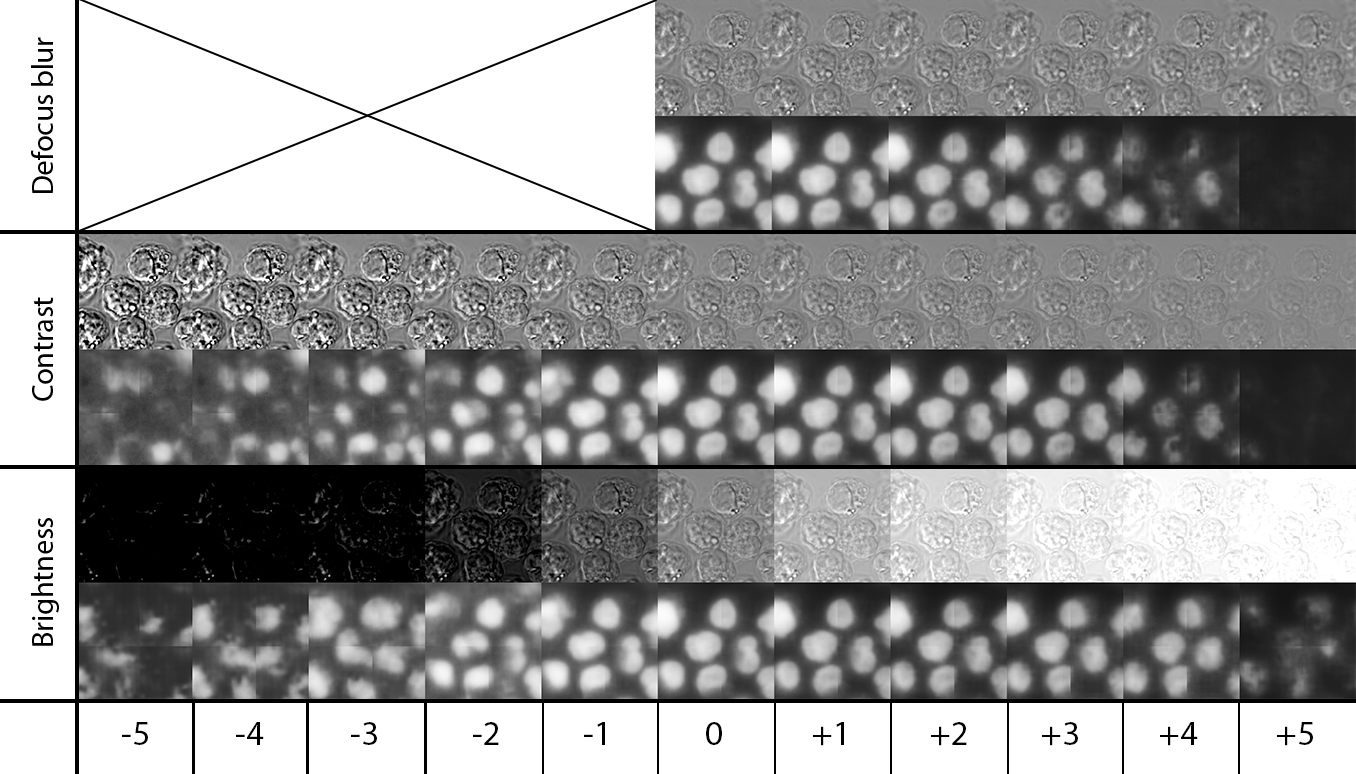
\includegraphics[width=0.5\linewidth]{bilder/corruptions.png}
		\caption{Influence of artificial corruptions on the predictions}
        \label{fig:artificial-corruptions}
	\end{center}
\end{figure}

One can observe the input image change for each of the corruptions along with the change of prediction of nuclei model in Figure \ref{fig:artificial-corruptions}. It can be clearly seen that the model's predictions are quite stable towards different brightness levels and contrast. However, the predictions on the crops are very sensible towards defocus blur corruption: DIC images with defocus blur levels $1-4$ are almost indistinguishable from the original image, yet the model's predictions degrade quite fast. This can be explained by the fact that the training dataset contains quite diverse data in terms of contrast and brightness levels and, as a result, the model is more stable towards these changes. Using defocus blur as an augmentation will help to solve this problem. This will be described in more detail in Section \ref{section:augments-againts-corruptions}.
\begin{figure}[htb]
	\begin{center}
		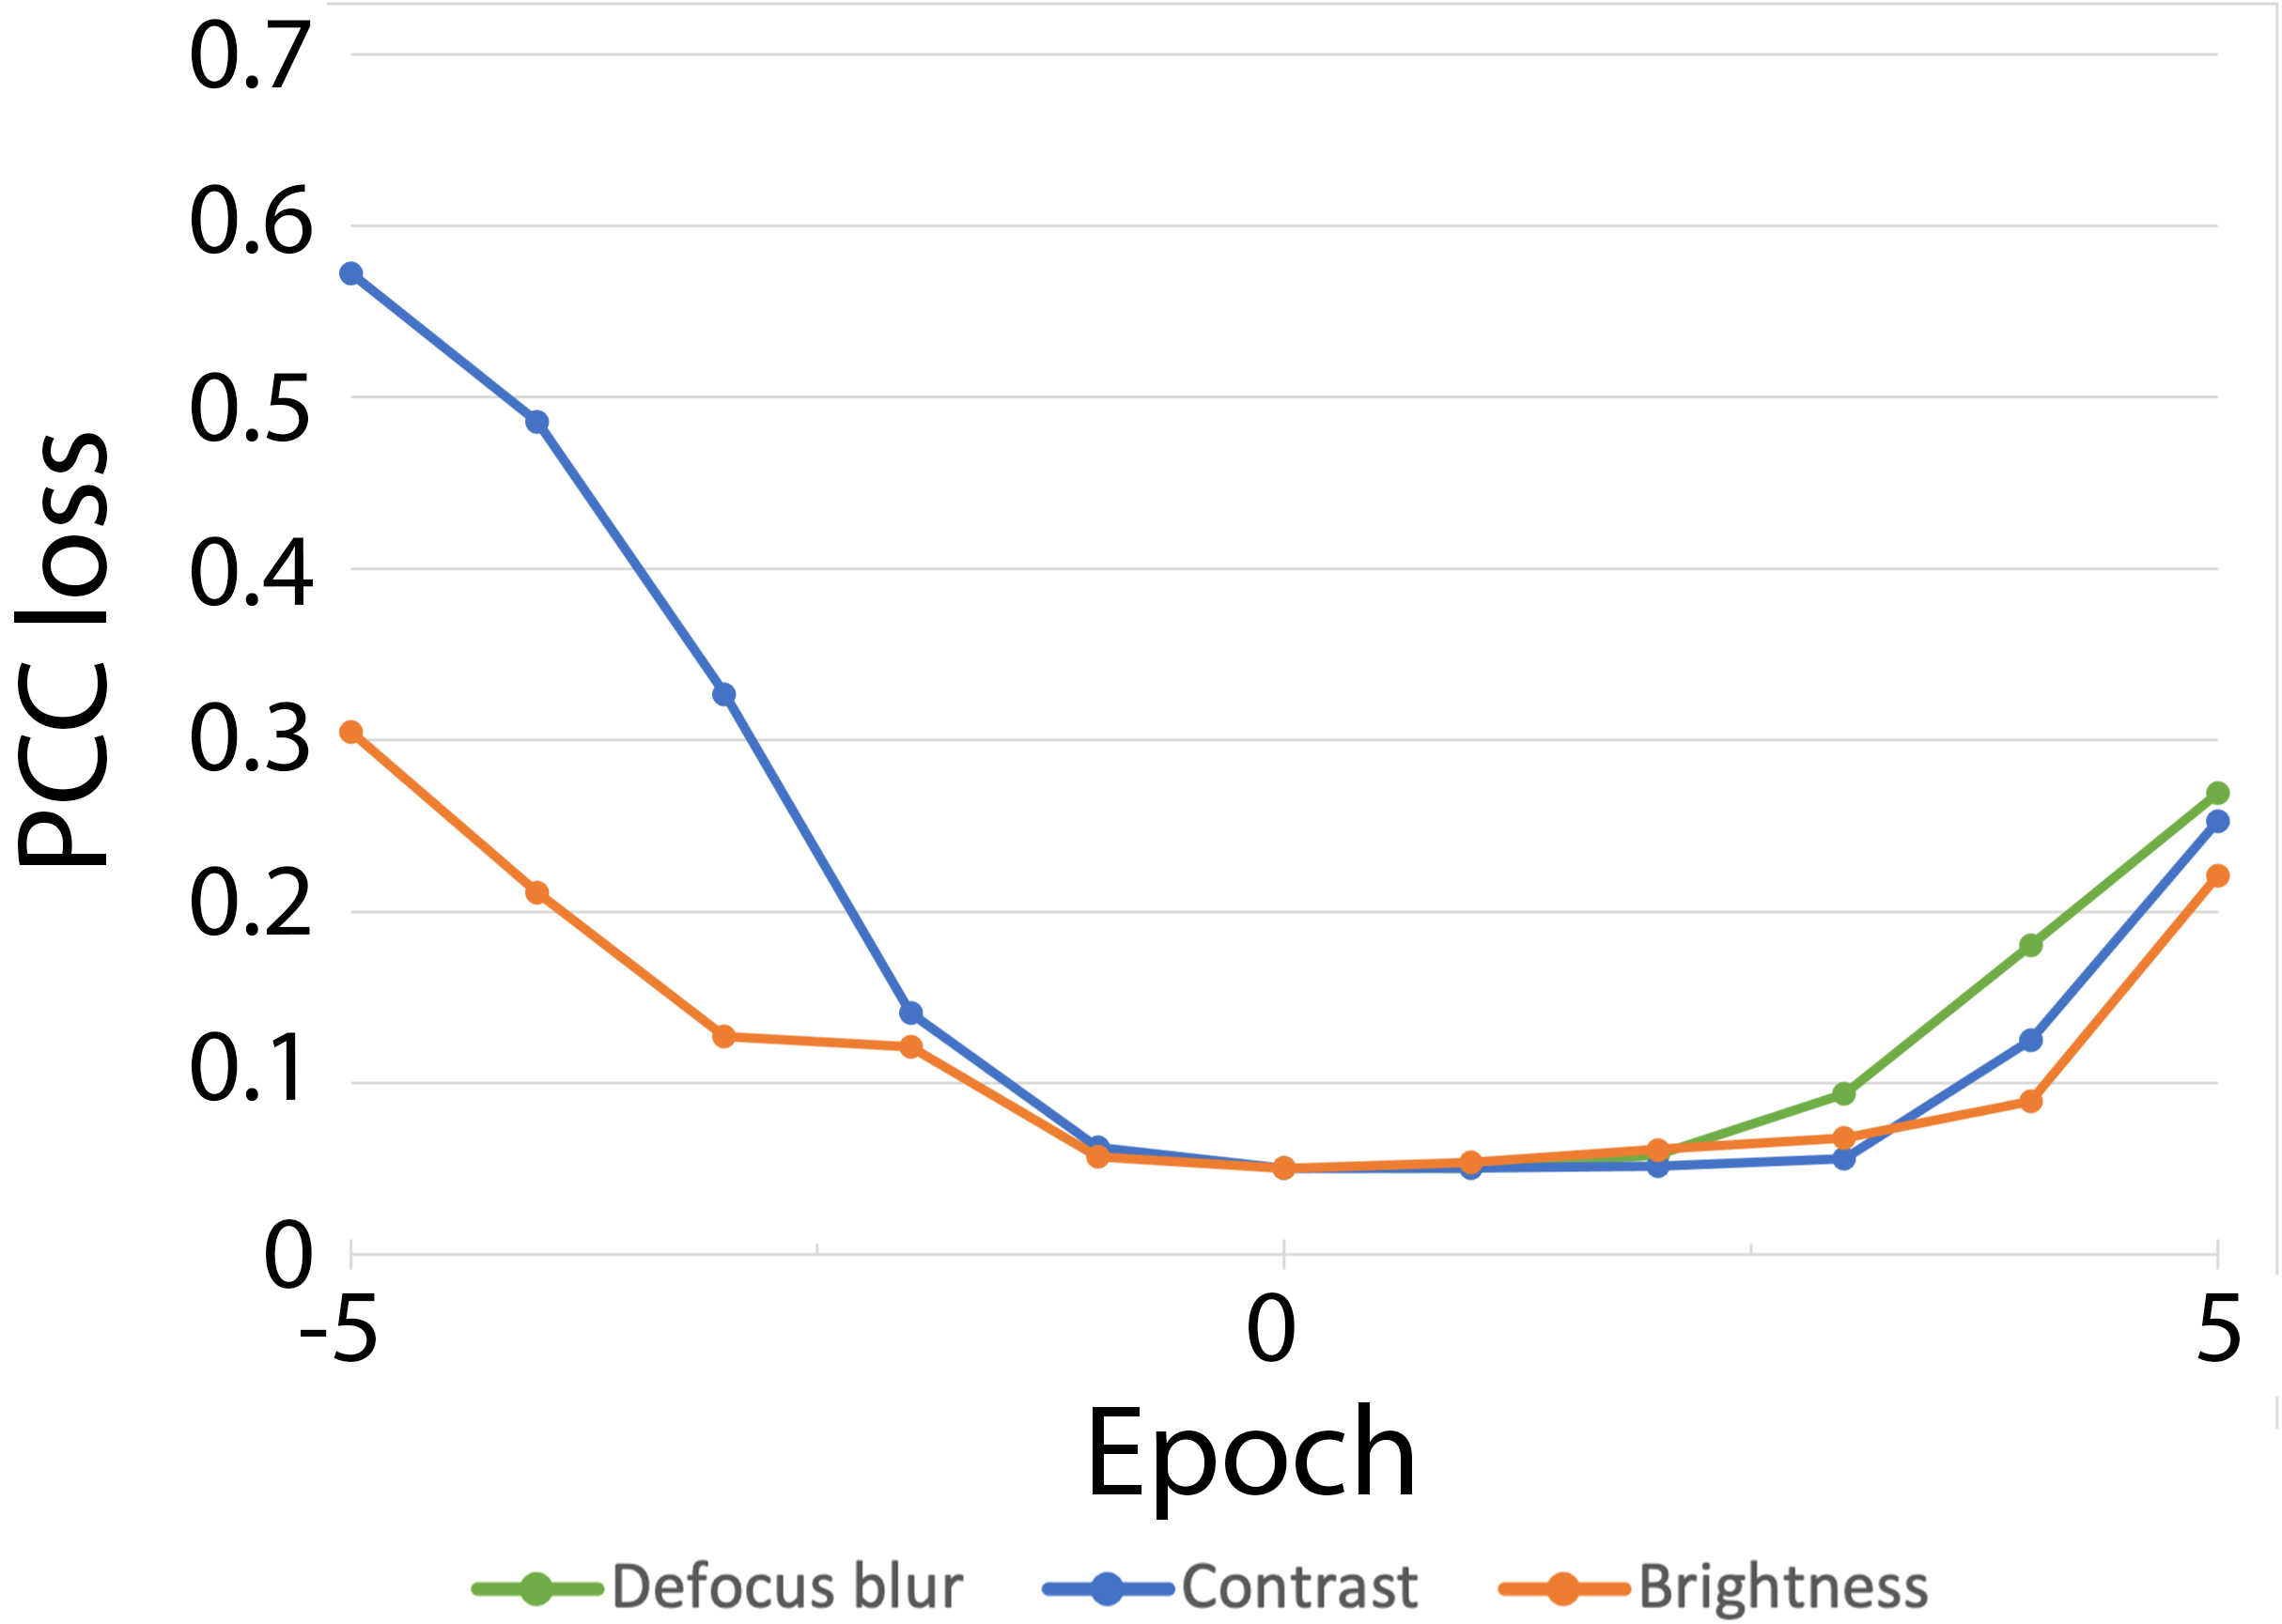
\includegraphics[width=0.5\linewidth]{bilder/corruptions-loss.png}
		\caption{Change of PCC loss for artificial corruptions}\label{fig:corruptions-loss}
	\end{center}
\end{figure}

Additionally, a change in PCC loss is presented in Figure \ref{fig:corruptions-loss}. This is a plot of PCC loss for different artificial corruptions. Loss increases for stronger severity levels. We can see that in a positive direction with defocus blur corruption the model degerates more quicker and that contrast corruptions change predictions more severely in the negative one.
    \subsubsection{Real corruptions}
        \label{section:real-corruptions}
        \paragraph{Not fixed cells imaging as corrupted input}
    \begin{figure}[H]
        \begin{center}
            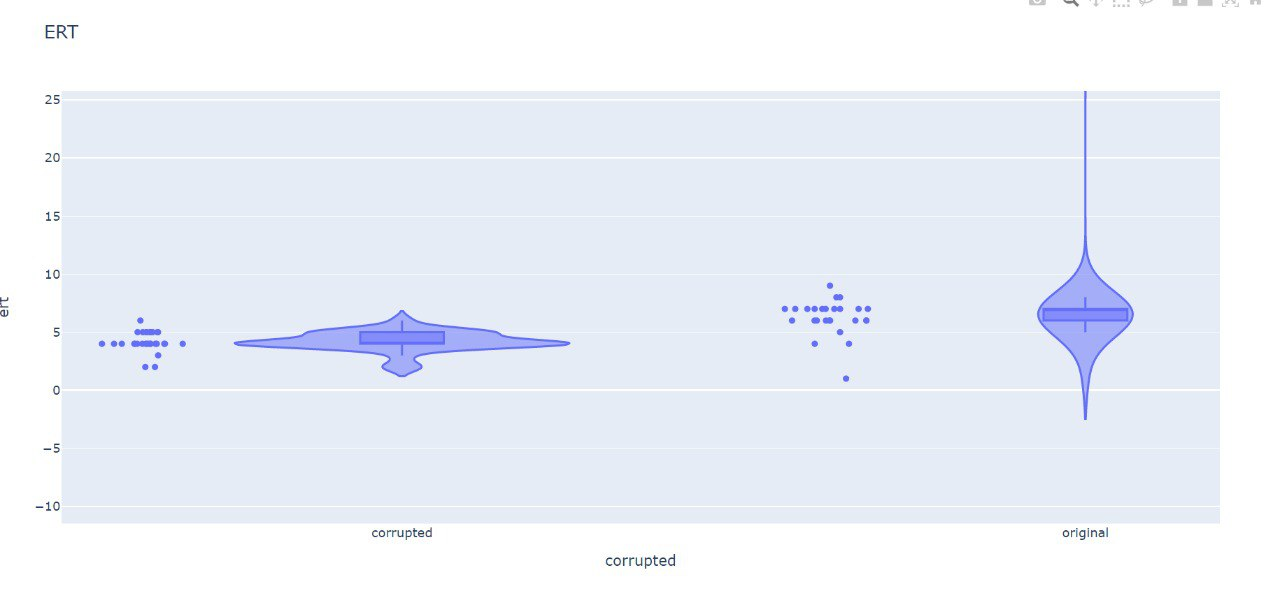
\includegraphics[width=0.5\linewidth]{bilder/drift-detection/online-fixed-vs-not-fixed.jpg}
            \caption{Online drift detection of not fixated cells}\label{fig:online-drift-not-fixed}
        \end{center}
    \end{figure}

    Scores of 0.91 however the threshold is 6, not corrupted data (fixed cells) mostly ert of 7 whereas corrupted data (not fixed cells) have an ert of 4. The threshold is therefore 6.

\paragraph{Real-world examples of corruptions}

    \subsubsection{Improving predictions with additional corruption augmentations}
        \label{section:augments-againts-corruptions}
        Going from observations of the models' stability towards different image brightness which is present in the datasets a new hypothesis was drawn. Introducing corruptions that we test on into the training should improve the predictions on corrupted data. Unfortunately, it is not possible to use real lab corruptions here as the data was provided only for testing on these difficult cases and was not stained. Without staining one cannot give a quantitative measure of the quality of the predictions. However, artificial corruptions can be applied here easily. Random changes in contrast, brightness and defocus blur of severity levels $-4$ and $4$ were added to the training augmentations. After the improved model was trained the predictions on the corrupted dataset became much better indeed (see Figure \ref{fig:augments-help}).

\begin{figure}[htb]
	\begin{center}
		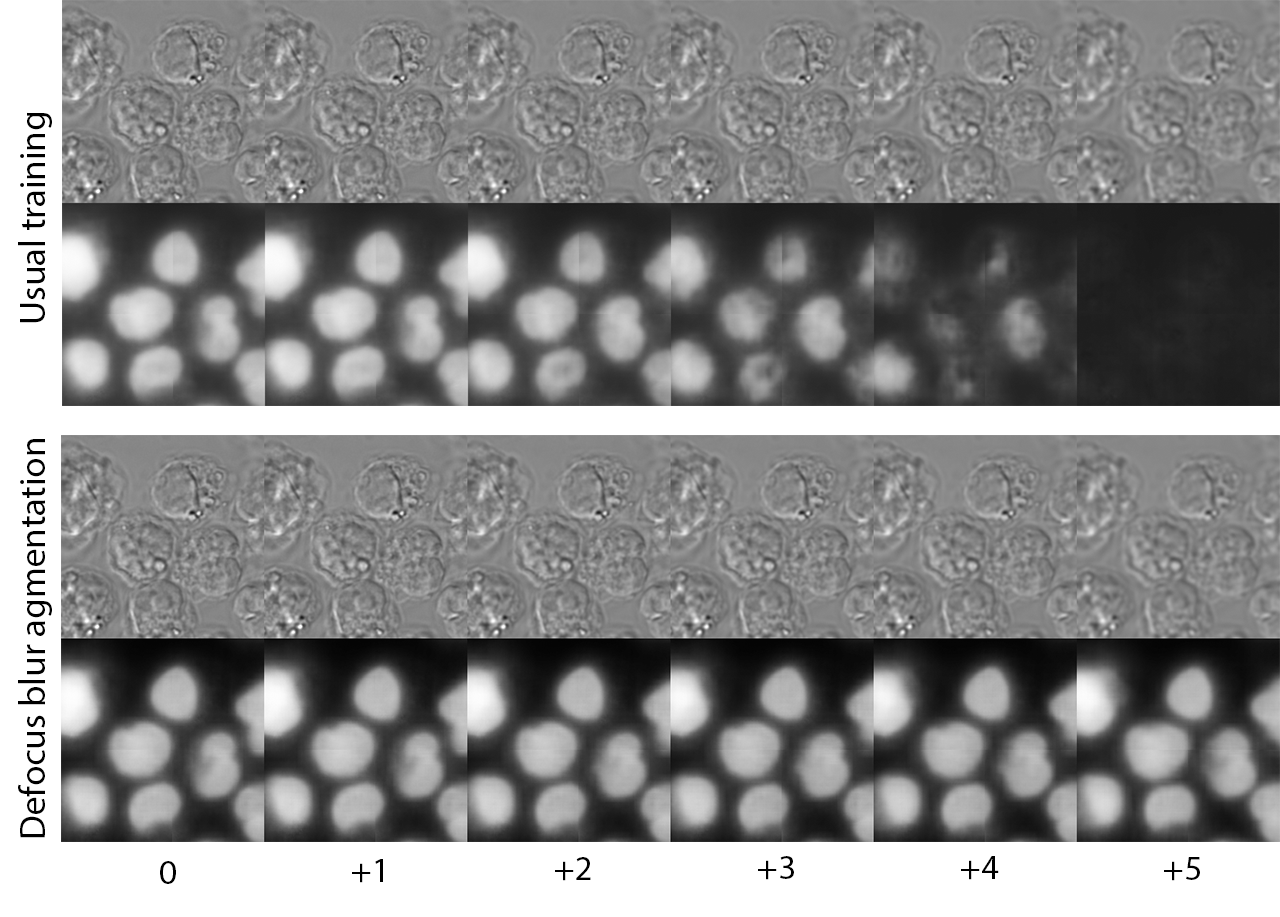
\includegraphics[width=0.4\linewidth]{bilder/stability/augments-help.png}
		\caption{Using corruptions as augmentations to improve predictions predictions}\label{fig:augments-help}
	\end{center}
\end{figure}

\subsubsection{Influence of corruptions on metrics for downstream tasks}
Additionally, since for artificial corruptions the ground truth data from staining is present, the difference in downstream metrics for models with and without augmentations was measured (see Table \ref{table:nuclei-corruptions-downstream-metrics-coefficients}), more specifically Spearman rank correlarion coefficients are compared. The calculation of downstream metrics remained the same except the thresholding algorithm was switched to a global one due to the time limit. This results in the wrong segmentation of some of the ground ground truth images. Therefore Spearman rank correlation coefficient is more repesentative here since it is more stable towards the outliers. The rest of the postprocessing procedure has remained the same apart from the application of artificial corruptions on the input data.

\begin{table}[htb]
    \centering
    \caption{Correlation coefficients for downstream tasks on nuclei}
        \begin{adjustbox}{width=0.7\linewidth}
            \begin{tabular}{|c|c|c|c|c|}\hline
                Contrast level&Number of nuclei&Total intensity&Mean intensity&Area\\\hline\hline
                +1&0.934&0.825&0.826&0.898\\\hline
                +2&0.932&0.820&0.819&0.899\\\hline
                +3&0.934&0.799&0.822&0.890\\\hline
                +4&0.804&0.439&0.671&0.540\\\hline
                +5&0.394&0.351&0.383&0.313\\\hline \hline
				Defocus blur level&Number of nuclei&Total intensity&Mean intensity&Area\\\hline\hline
                +1&0.934&0.832&0.827&0.905\\\hline
                +2&0.929&0.800&0.820&0.890\\\hline
                +3&0.934&0.756&0.8210&0.871\\\hline
                +4&0.838&0.361&0.666&0.501\\\hline
                +5&-0.072&-0.233&-0.231&0.07\\\hline
            \end{tabular}
        \label{table:nuclei-corruptions-downstream-metrics-coefficients}
        \end{adjustbox}
\end{table}

One can observe from the table above that the metrics degrade quite fast starting from the severity level $3$. The most affected metrics are the total and mean intensity. The number of organelles seems to be the most stable one until the very last severity level when the predictions turn almost completely black. 
    \subsubsection{Generalizability across phenotypes}
        TODO train the model on one phenotype and predict on the other, compare predictions (visually?)
        postprocessing with metrics then?
    \pagebreak
    \subsection{UNET embeddings study}
    Similarly to studying autoencoder embeddings that represent a high-dimentional input in lower dimentional space, one can study UNet embeddings. However, it is important to keep in mind that the dimensionality of embeddings in UNet case is not lower than dimensionality of the input and is even often higher (see the UNet architecture in Figure \ref{fig:unet}). The goal of a UNet in contrast to an autoencoder is not to compress the input, but to extract useful features that are helpful for high-resolution segmentation. UNet embeddings do not contain rich image semantics in them as embeddings of an autoencoder do. UNet compresses the spatial dimention of the input, but at the sme time it gradually increases the number of filters that capture of information need for segmentation. As it has been proven in section \ref{section:nuclei-predictions} having more filters only helps to get better predictions, therefore there is no need for a UNet to have low-dimentional embeddings. Nevertheless, it is still interesting to see if the embeddings do contain any information about the input that one could use. There were two hypothesis put in question: the first one is whether embeddings of a trained UNet form any kind of clusters based on cells phenotype. And a second one is whether embeddings of corrupted images can be clustered together further away from not corrupted ones. If the latter hypothesis would hold, one could alarm the end-user about the outliers in the dataset based on their distance from both of the clusters. 
    \subsubsection{Application of various dimentionality reduction methods}
        \label{section:unet-embeddings-dim-reduction}
        \begin{figure}[H]
	\begin{center}
		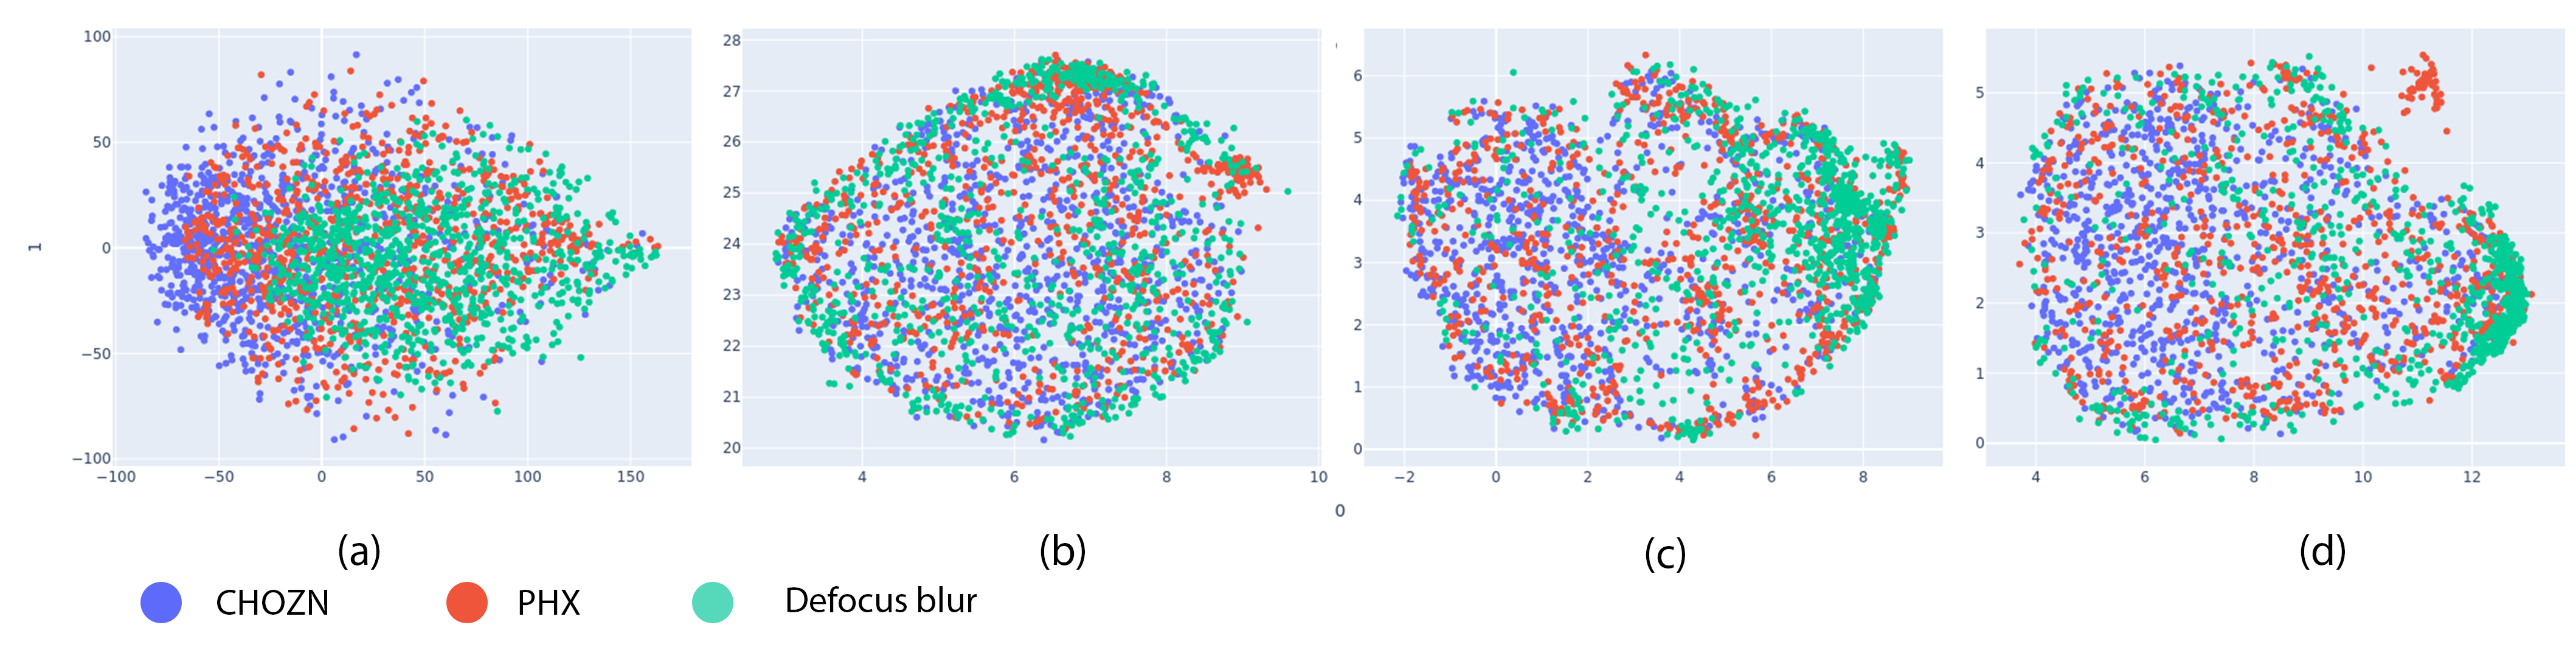
\includegraphics[width=\linewidth]{bilder/unet-embeddings/umap-pca-embeddings.png}
		\caption{(a) PCA, (b) UMAP, (c) combination of PCA and UMAP with 10 and (d) 50 components}\label{fig:umap-pca-embeddings}
	\end{center}
\end{figure}

    \subsubsection{Autoencoder embeddings as an alternative}
        Since UNet embeddings do not seem to exhibit any exceptional results in terms of clustering, it was decided to train an autoencoder directly on DIC image crops. Since the autoencoder's embeddings contain dense semantic information of the input they might provide more insights for clustering the previously mentioned hypotheses. Figure \ref{fig:ae-training} presents the architecture of two convolutional autoencoders used for these experiments. One compresses $256 \times 256$ input crops into embeddings vector of size $3528$ and another one compresses them into a vector of a smaller size of $200$. Both autoencoders were trained using MSE loss. The results of their convergence are presented in Figure \ref{fig:ae-training} on the right.

\begin{figure}[H]
	\begin{center}
		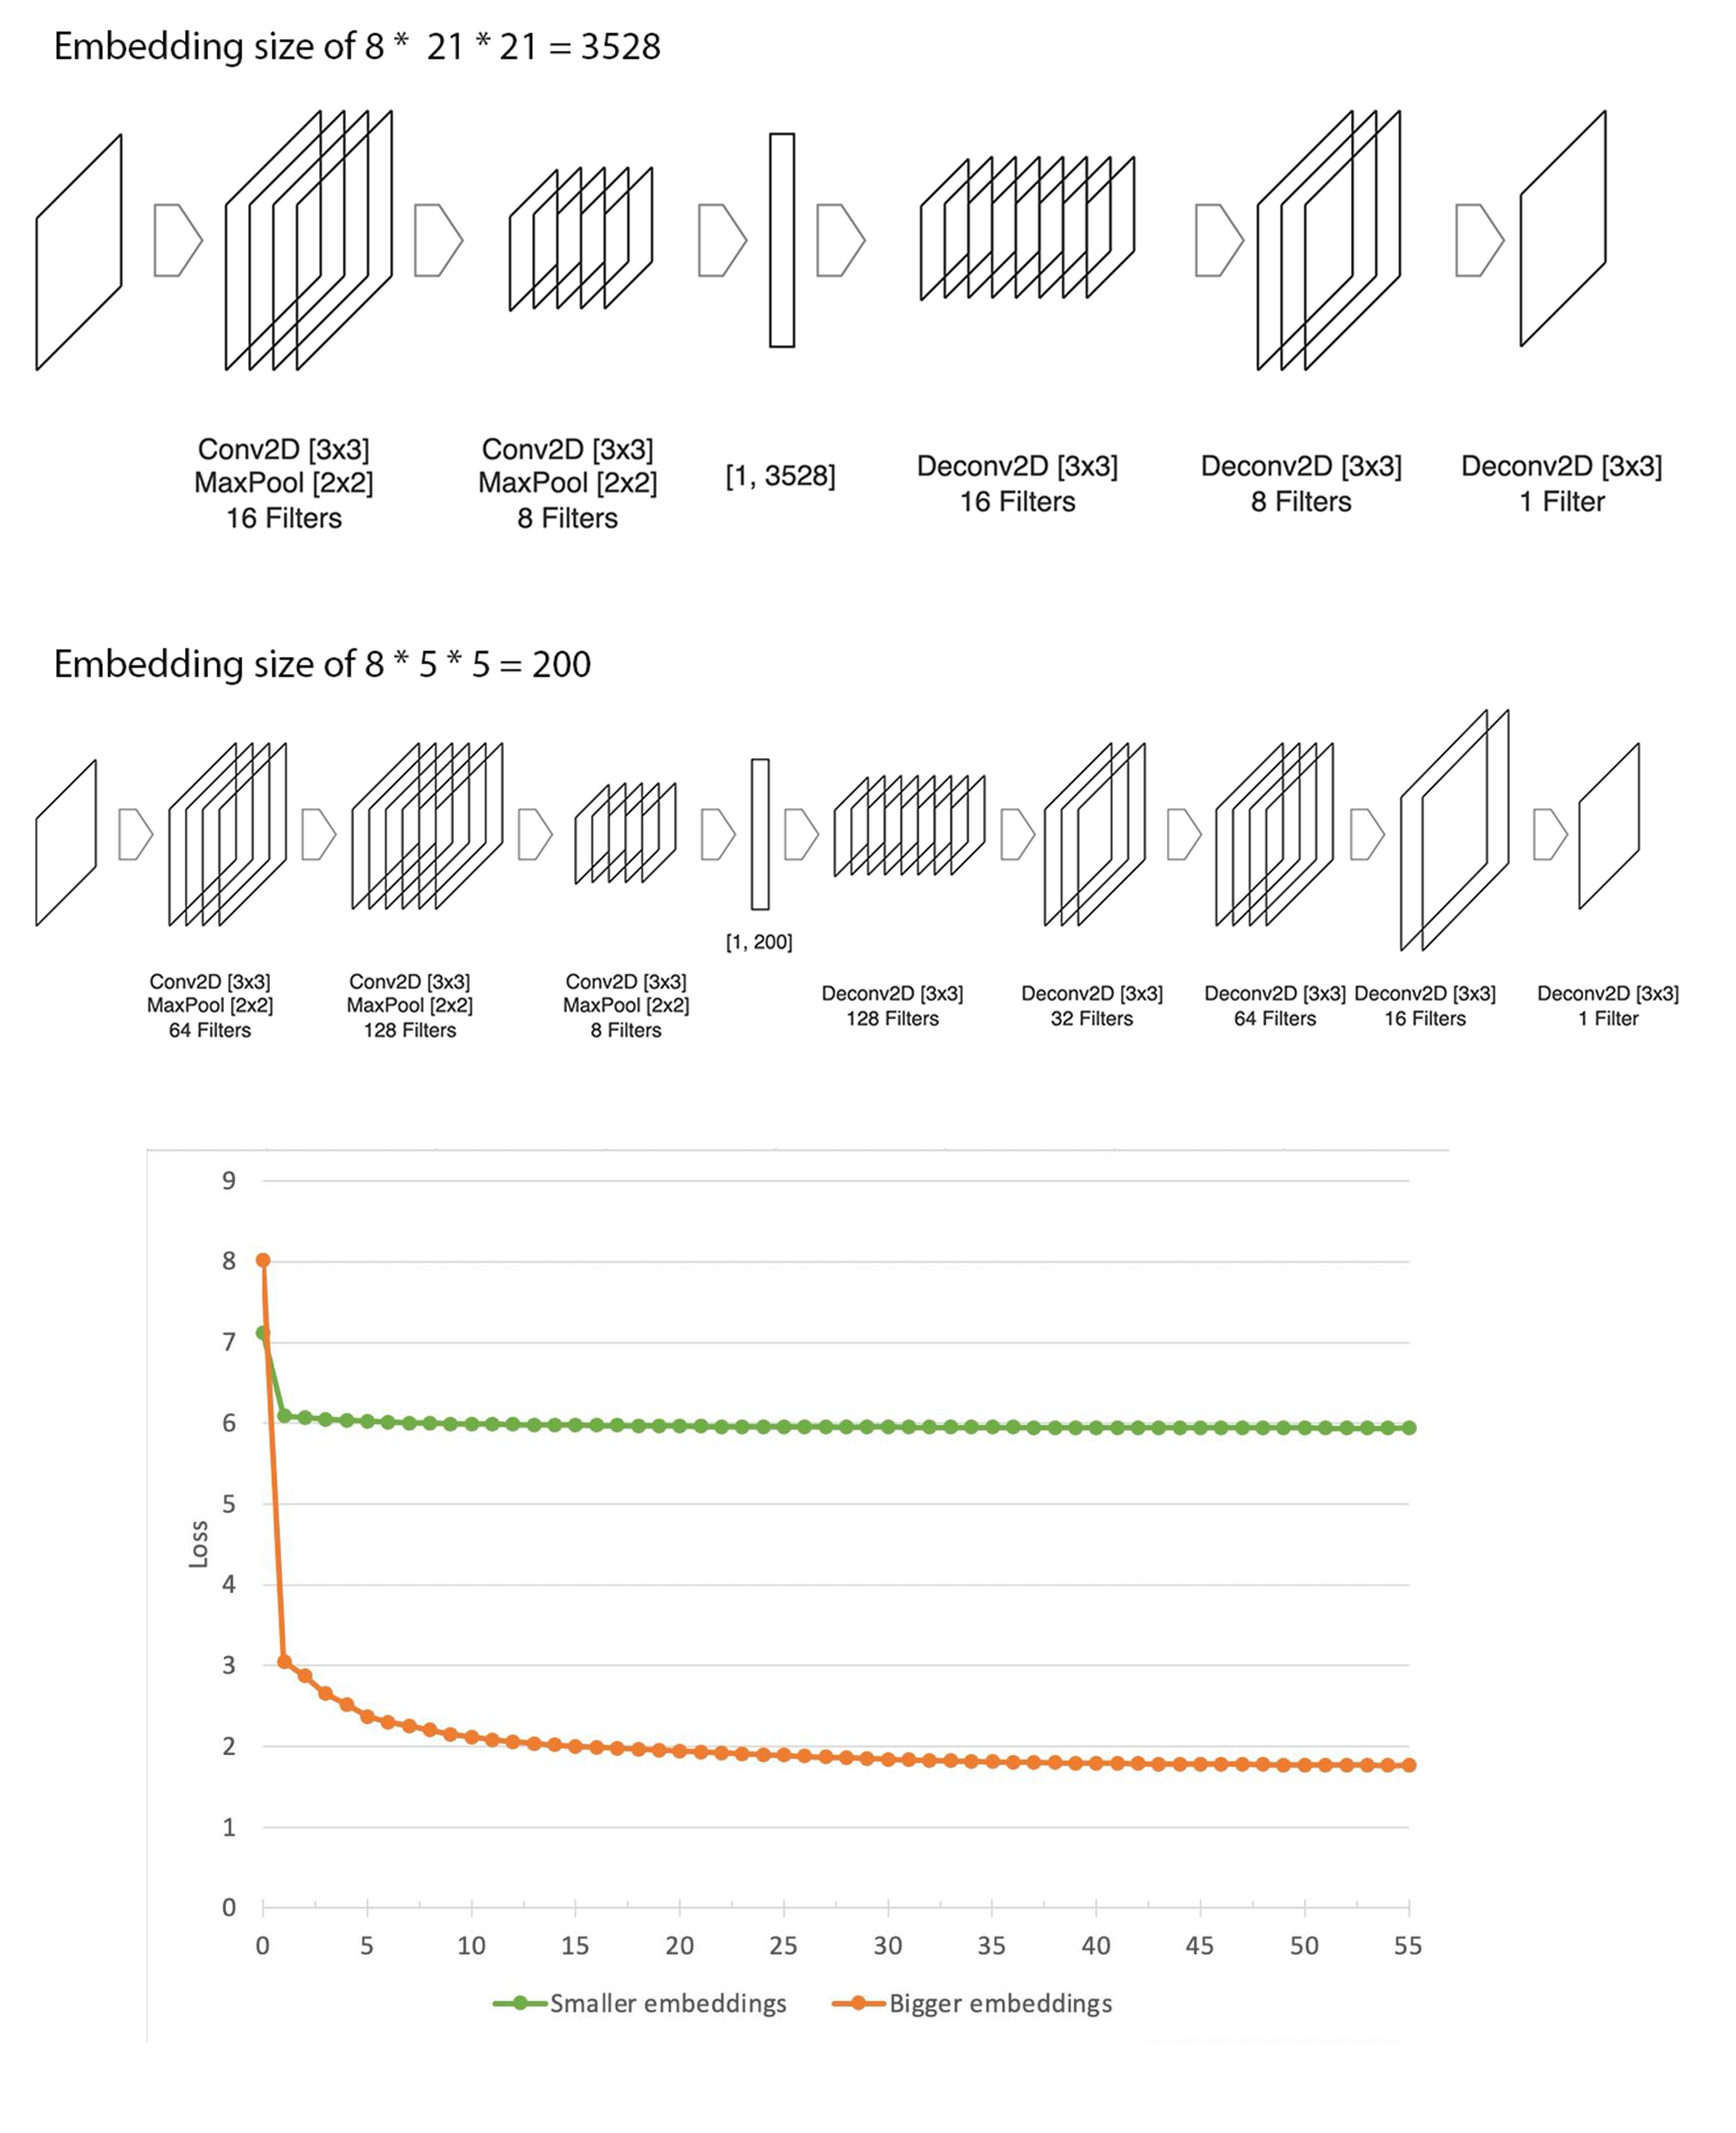
\includegraphics[width=\linewidth]{bilder/ae-embeddings/training-architectures.png}
		\caption{Architectures of two autoencoders and their training convergence}\label{fig:ae-training}
	\end{center}
\end{figure}

An autoencoder with embeddings of bigger size was able to achieve a lower loss as well and the samples reconstructed from it were of higher quality (see Figure \ref{fig:ae-samples}). Clearly reconstruction of the samples will not have a high resolution as there are no skip-connections in this architecture. However, this is also not needed, the main goal here is to find out whether autoencoder embeddings provide any insights on the data.
\begin{figure}[htb]
	\begin{center}
		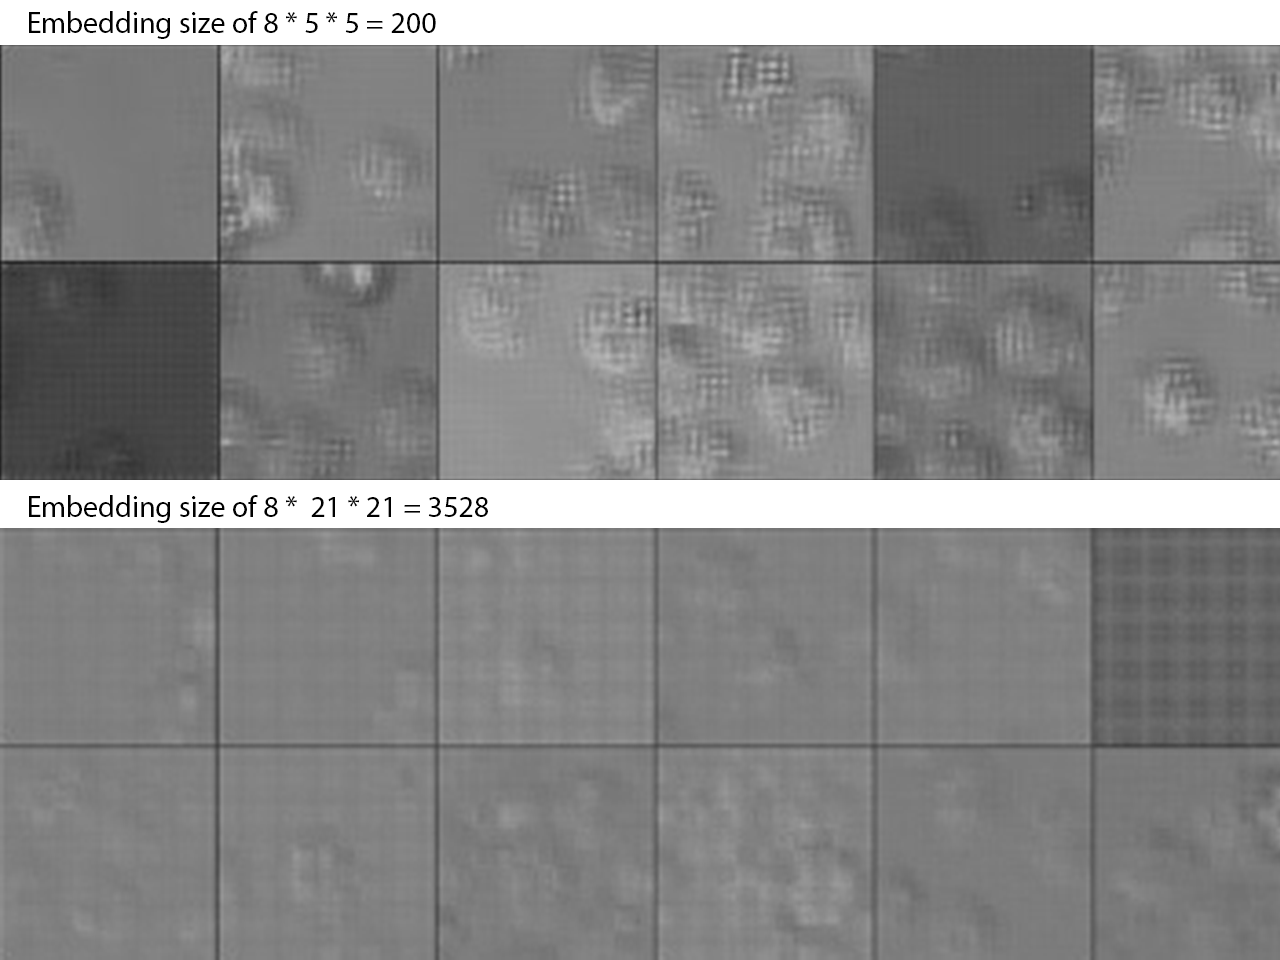
\includegraphics[width=0.5\linewidth]{bilder/ae-embeddings/ae-samples.png}
		\caption{Samples drawn from trained autoencoders. (a) --- an autoencoder with a smaller bottleneck layer, (b) --- an autoencoder with a bigger bottleneck layer}
		\label{fig:ae-samples}
	\end{center}
\end{figure}

Since an autoencoder with bigger embedding size seems to be able to reconstruct crops much better we have proceeded with its architecture. Embeddings were projected into a two-dimensional space using first PCA with 10 components and then applying UMAP on PCA's projections. The results of such projection are presented in Figure \ref{fig:ae-pca-umap-clustered}. Two clearly defined clusters appear: the left plot presents projections from an earlier epoch, the right one from a later one. Embeddings separate gradually into two clusters throughout the training.

\begin{figure}[htb]
	\begin{center}
		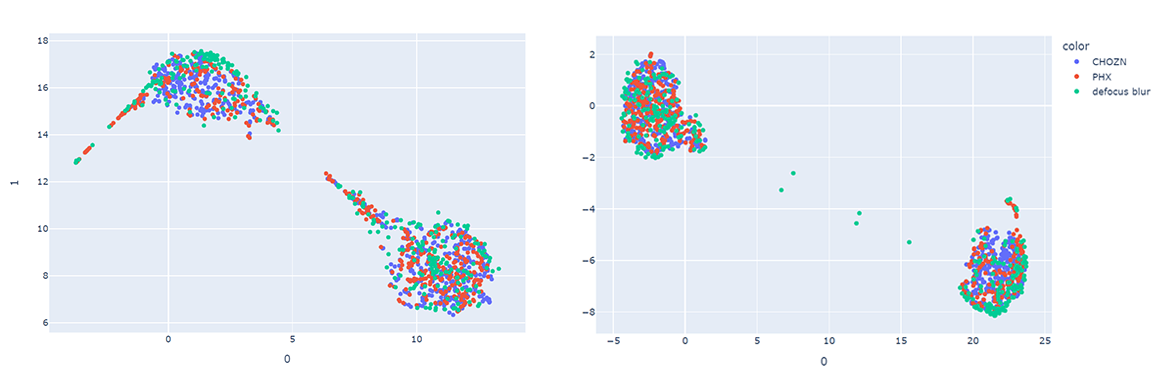
\includegraphics[width=0.5\linewidth]{bilder/ae-embeddings/pca-umap-clusters.png}
		\caption{Autoencoder embeddings after applying PCA and UMAP afterwards}\label{fig:ae-pca-umap-clustered}
	\end{center}
\end{figure}

However, these two clusters are based neither on cell phenotypes nor on input corruption. All points of both phenotype as well as corruptions seem to be equally spread between two clusters. By looking at the images corresponding to each of the clusters it soon becomes apparent that the main difference between them is their brightness level.  To prove this theory distributions of average image intensity of images in both clusters are presented in Figure \ref{fig:ae-brighter-darker}. In the violin plots we can see that the distribution of the crops on the left has a much lower brightness level than the distribution of the crops on the right. However, it is hard to account for why the brightness were different, it might happed due to many different reasons, for example, the images might have been taken on different days when the microscopy lighting conditions might have been different.
%\begin{figure}[htb]
%	\begin{center}
%		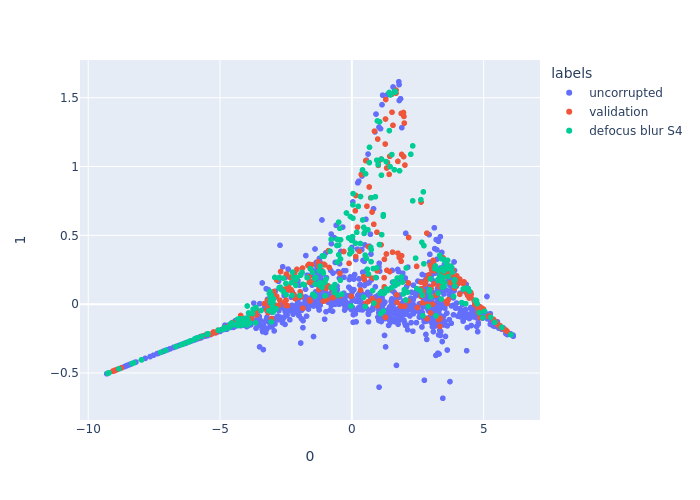
\includegraphics[width=0.5\linewidth]{bilder/ae-embeddings/pacmap.png}
%		\caption{PacMAP does not provide information on the coruption}\label{fig:ae-pacmap}
%	\end{center}
%\end{figure}

\begin{figure}[htb]
	\begin{center}
		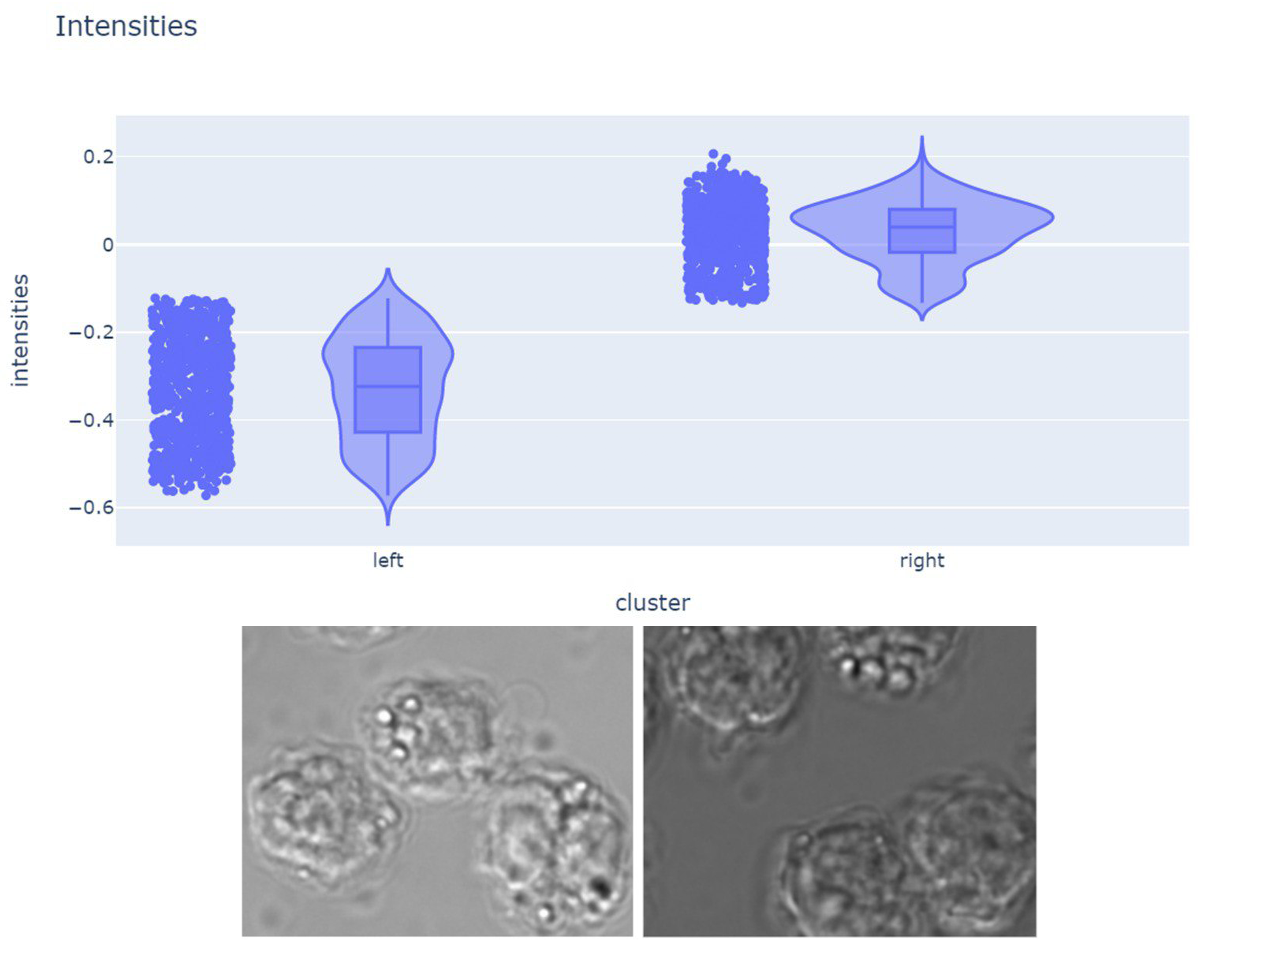
\includegraphics[width=0.5\linewidth]{bilder/ae-embeddings/brighter-darker.png}
		\caption{Different in brightness in the clusters formed by an autoencoder embeddings in a two-dimensional space}
		\label{fig:ae-brighter-darker}
	\end{center}
\end{figure}

Since an autoencoder picks up on brightness difference within the crops, it is worth trying to normalize crop brightness across the entire dataset first. Nevertheless, it is not a trivial task as images have different cell density in them. This is why some images that contain primarily background pixels will always be darker than the ones that contain enough of foreground. We suggest to filter the crops based on the amount of cell criteria (which can be done using GFP model that can detect cells present in DIC) and normalize them afterwards. Retraining the autoencoder with new training data might provide more insights when the difference in brightness is gone.

It is also clear why autoencoder embeddings do not provide any clustering for corrupted crops. Corruption severities neither really change the image semantics nor are they significantly different visually speaking (see defocus blur in \ref{fig:artificial-corruptions}). Therefore they do not alter the ability of an autoencoder to restore input correctly. In contrast, UNet's fluorescence predictions do suffer significantly for several corruption levels, its predictions strongly change --- the outline of organelles becomes more blurry, additional shine appears in fluorescence prediction. These changes happen not only during the decoding part, but they also might bring unsual values in the embedding representation. Therefore UNet embeddings have more information on the "trustworthiness" of predictions. That is why when defocus corruptions are used as training augmentations, drift detection for the model trained with these corruptions stops alarming about the drift. Even though it did for the model, which did not have these augmentations present [TODO add section reference]. This happens simply because the models' predictions degrade and start looking different, which triggers a "drift alarm". With the improved predictions, drift alarm would not be triggered even when using the same data.
    \subsubsection{Clustering of PaCMAP embeddings}
        \paragraph{Clustering on UNet embeddings}
        \label{section:clustering-on-unet-embeddings}
        Since the UNet embeddgins are the most promising for clustering based on input corruptions we will proceed with this approach. Apart from dimensionality reduction methods used in section \ref{section:unet-embeddings-dim-reduction}, PaCMAP clustering was tried. You can find its detailed description in section \ref{section:pacmap}. 
\begin{figure}[htb]
	\begin{center}
		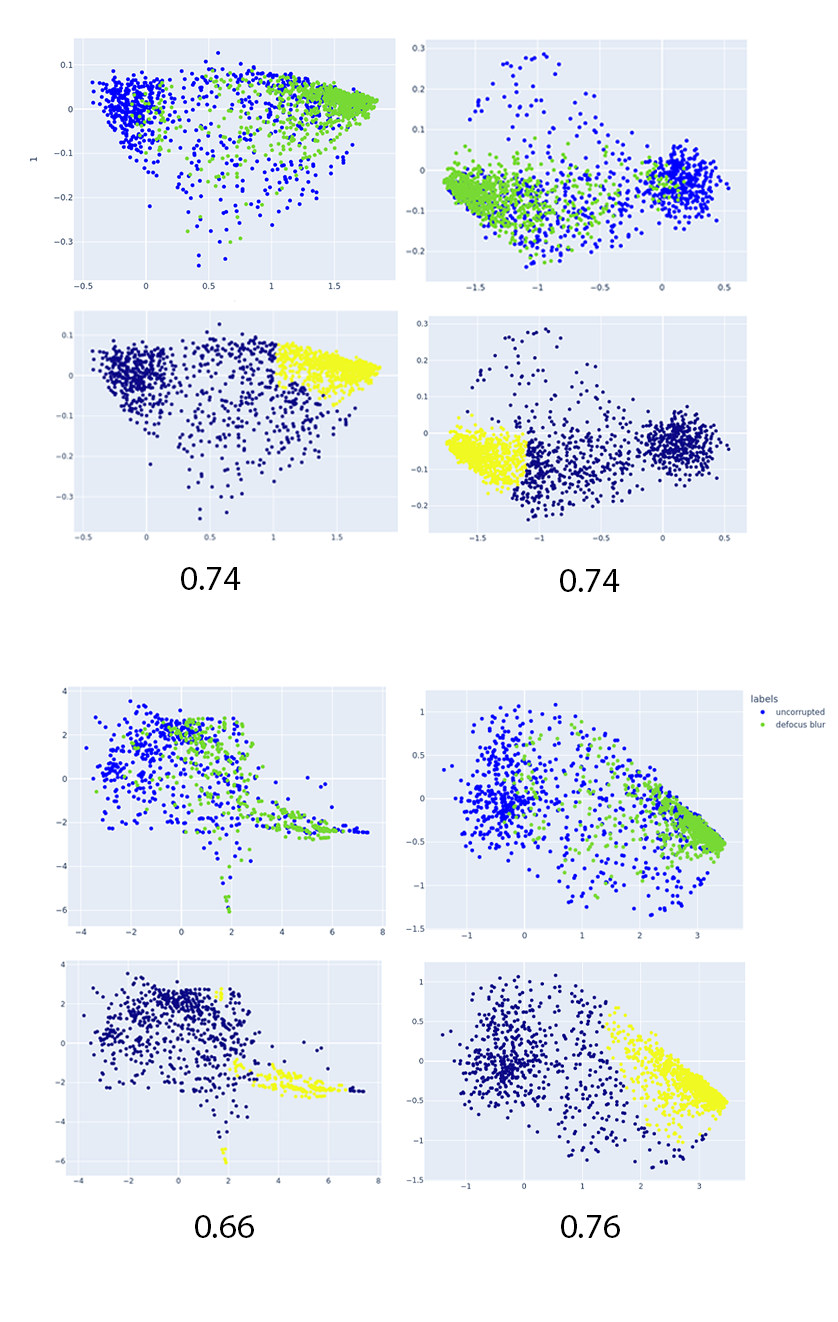
\includegraphics[width=\linewidth]{bilder/unet-embeddings/PacMAP.png}
		\caption{Clustering of UNet embeddings after PacMAP}
		\label{fig:unet-clustering}
	\end{center}
\end{figure}

PaCMAP allows a more flexible hyperparameter tuning in order to preserve local and global relations from high-dimentional data and as result a better clustering can be found. As usual PaCMAP was trained using "good" training data only, meaning no corruptions were introduced. And only when the transformation from high-dimensional into a lower dimensional space was found, corrupted crops were projected using this transformation. Figure \ref{fig:unet-clustering} presents results of training PaCMAP with 4 different hyperparametrization settings. There are 3 hyperparameters that were changed here: MN\_ratio, FP\_ratio and n\_neighbors. Detailed explanation of their influence was also described in section \ref{section:pacmap}. From left to right in Figure \ref{fig:unet-clustering}:

\begin{itemize}
	\item MN\_ratio=0.5, FP\_ratio=0.1, n\_neighbors=10
	\item MN\_ratio=0.1, FP\_ratio=0.1, n\_neighbors=10
	\item MN\_ratio=0.5, FP\_ratio=0.5, n\_neighbors=2
	\item MN\_ratio=0.1, FP\_ratio=0.5, n\_neighbors=10
\end{itemize}

In this case cluster of green dots represents projected UNet embeddings of images corrupted with defocus blur with severity level $4$, which is already a strong corruption and leads to unacceptable predictions of the model, that did not have defocus blur augmentations. However, these point are still strongly mixed with not corrupted ones. In order to check how separable they are unsupervised clustering DBSCAN alogorithm was used. Results of this clustering are shown in Figure \ref{fig:unet-clustering-sev-levels}. Density based clustering approach used here was described in details in section \ref{section:dbscan}. 

\begin{figure}[htb]
	\begin{center}
		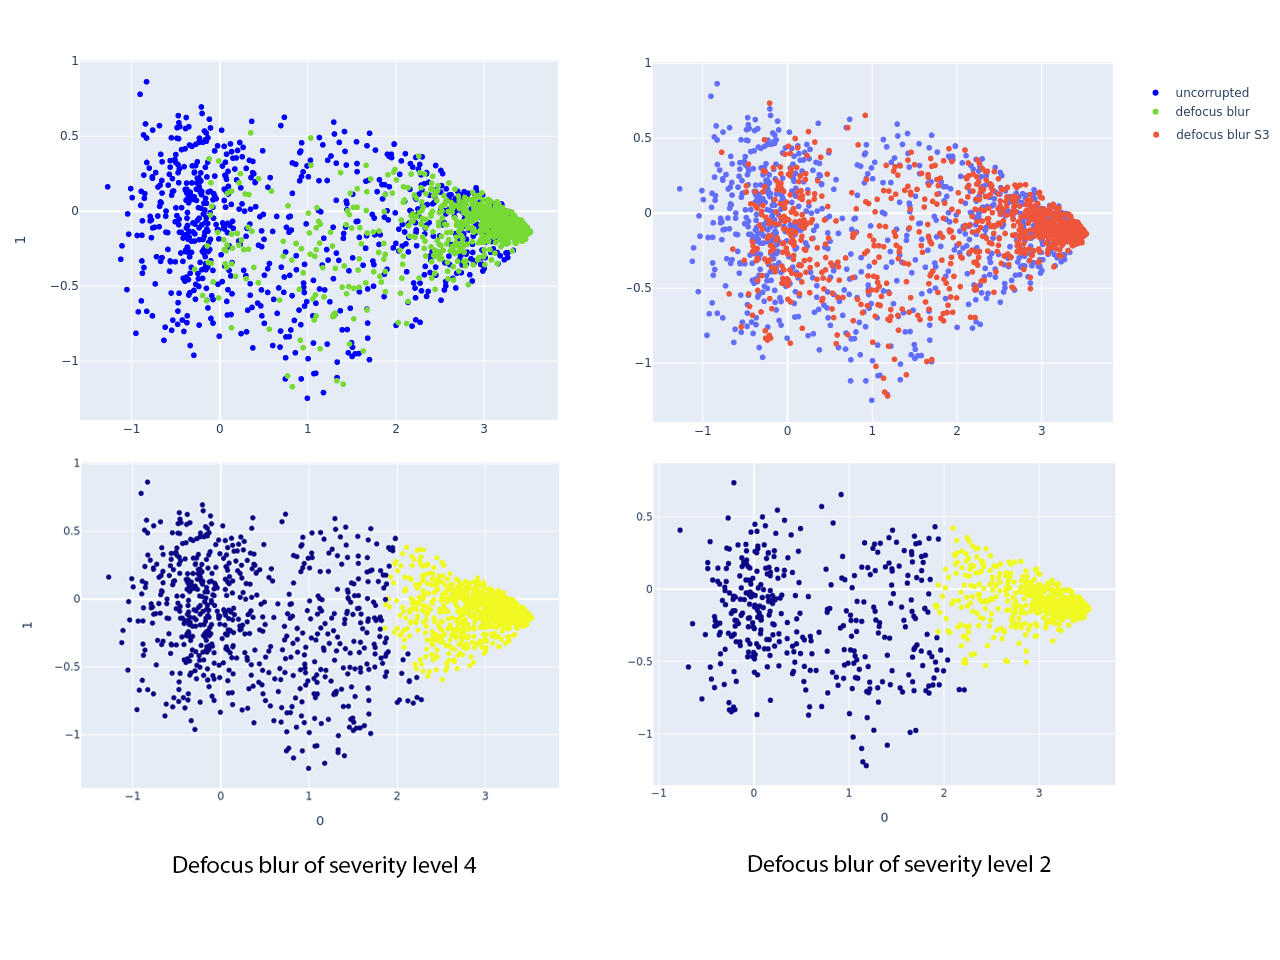
\includegraphics[width=0.6\linewidth]{bilder/unet-embeddings/db-levels.png}
		\caption{Clustering of UNet embeddings after PacMAP for different severities levels}
		\label{fig:unet-clustering-sev-levels}
	\end{center}
\end{figure}

After training DBSCAN on not corrupted crops embeddings it has recognized a class on the right (yellow dots) as a cluster and the rest of the points (blue ones) as noise, because they have quite low density in comparison to the yellow cluster. This is not a problem if we consider noisy points simply as a separate cluster. For such clustering defocus blur of level $4$ splits the crops between two clusters with an F1-score of $0.74$. In Figure \ref{fig:unet-clustering-sev-levels} on the right red points represent projection of image embeddings after corrupting them with a defocus blur of severity level $3$. In this case they are mixed with not corrupted projections even stronger. Here prediction of already trained DBSCAN drops to F1-score of $0.64$.

Overall UNet embeddings do express clustering of corrupted embeddings to a small extent, however not strongly enough to use it in practice. Autoencoder here would be a better approach, however brightness normalization has to take place first. It is recommended to proceed the research here in the direction of contrastive learning algorithms, specifically \cite{csi} approach.
    \subsubsection{Embeddings for direct stability prediction}
        The problem of substituting fluorescence labeling with \textit{in silico} prediction solved in thesis is a step towards a general goal of the project within Merck KGaA oriented towards predicting cell stability and productivity. Instead of a usual feature analysis of sizes of cell organelles, their fluorescence intensities and quantities, one can incorporate feauture representations created by UNet directly into the pipeline for productivity predictions that uses assay features as its inputs (see Figure \ref{fig:productivity-fluroescence}).
\begin{figure}[htb]
	\begin{center}
		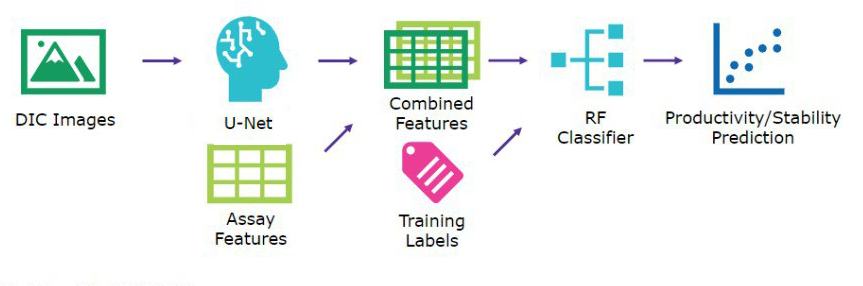
\includegraphics[width=\linewidth]{bilder/unet-embeddings/producitvity.png}
		\caption{Predicting productivity with fluorescence data incorporated}
		\label{fig:productivity-fluroescence}
	\end{center}
\end{figure}

Meaning that instead of training a model directly on assay features that are potentially providing information to predict future cell stability, one could combine them with the embeddings of a UNet model. Embeddings represent a rich representation of cells in DIC that has information on features needed for detecting cell organelles, therefore they might include other useful knowledge that was not analysed in the lab before and can be potentially useful for cell analysis. Most probably assay features will be combined with several UNet embeddings, as several different models were trained to predict different targets, however it would be possible to train a signle UNet model that would predict all targets at once, that will ensure even more informationally rich embeddings. Afterwards, with the help of random forest classifier productivity and stability rates can be derived. 

This approach has a strong theorectical portential behind it and requires acquiring stability and productivity data first to have a proof of concept. Since data acquisition in for this task requires more than 9 months, therefore the experiments could not be held within the scope of this work, but will be researched in the nearest future.
    \pagebreak
    \subsection{Drift detection}
    \subsubsection{A need to detect drift}
    \subsubsection{Maximum mean discrepancy for drift detection}
        \begin{figure}[H]
	\begin{center}
		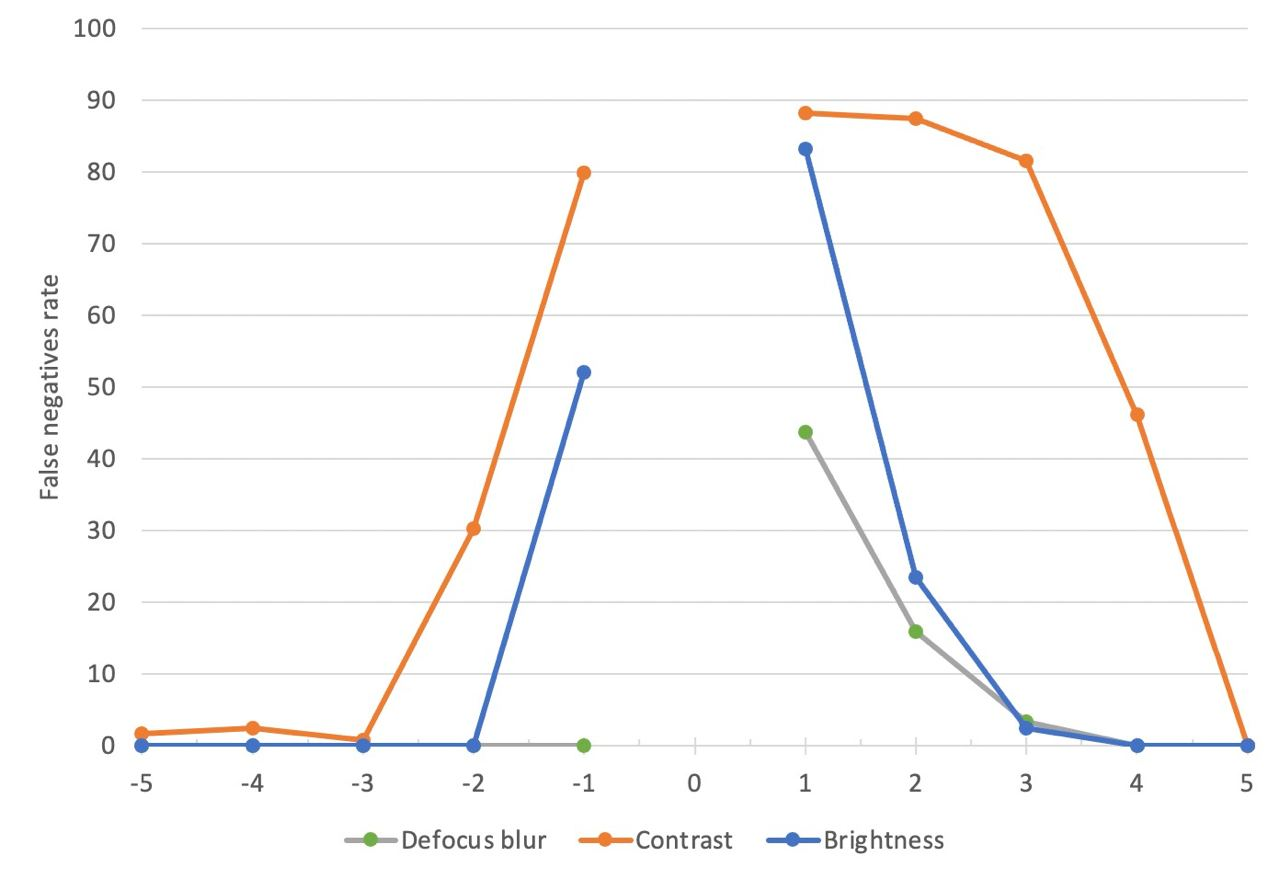
\includegraphics[width=0.5\linewidth]{bilder/drift-detection/fn-rate.jpg}
		\caption{False negatives rate for drift detection on artificial corruptions}\label{fig:fn-rate}
	\end{center}
\end{figure}
    \subsubsection{Online version of MMD algorithm}
            MMD algorithm in \textit{alibi-detect} library has an online version, which also presents an interest for our case. One of the main differences of an online drift detector is that it does not accept several inputs at once alerting whether they represent a drift all together, but it focuses on a single input at a time during its run. It assumes that there is a big dataset of reference data, that can be used as an example of a "correct" distribution and processes one embedding at a time. This single input would be sent into a test window where two-sample test-statistics (MMD essentially in this case) will be calculated. As soon as the test-statistic exceeds some pre-defined threshold a drift alert is send to the user. Apart from the threshold one has to define a so-called expected run-time (ERT). This time states how many inputs the detector should process on average before it makes a detection (false positive or true positive depending on which distributions the inputs were taken from). Another hyperparameter here is hidden in a size of a test-window. Becase the larger the window is, the more chance is there to detect a very slight drift, yet with a smaller window one gets a much faster response to severe drift. 

It is usually recommened to reduce the dimensionality of the data before feeding it into the algorithm. But in this case the performance was exceptional even for high-dimensional embeddings of the UNET model. Nevertheless, there are also options on how to reduce the dimensionality of the data from the authors of the framework.

This algorithm was trained on the same uncorrupted training data sent through the embeddings of a nucleus UNet. Yet, test crops are fed into a detector in a consecutive way --- in case of no corruptions present it is not enough to feed only several crops from one image, as the algorithm requires more data to be fed into the detector until it makes a decision. For example, ERT of not corrupted inputs can be even up to $180$ crops until a detector alerts a false positive detection. On the contrary for corrupted inputs drift detector needs normally $\leq 6$ crops (see Figure \ref{fig:online-ert})
\begin{figure}[H]
	\begin{center}
		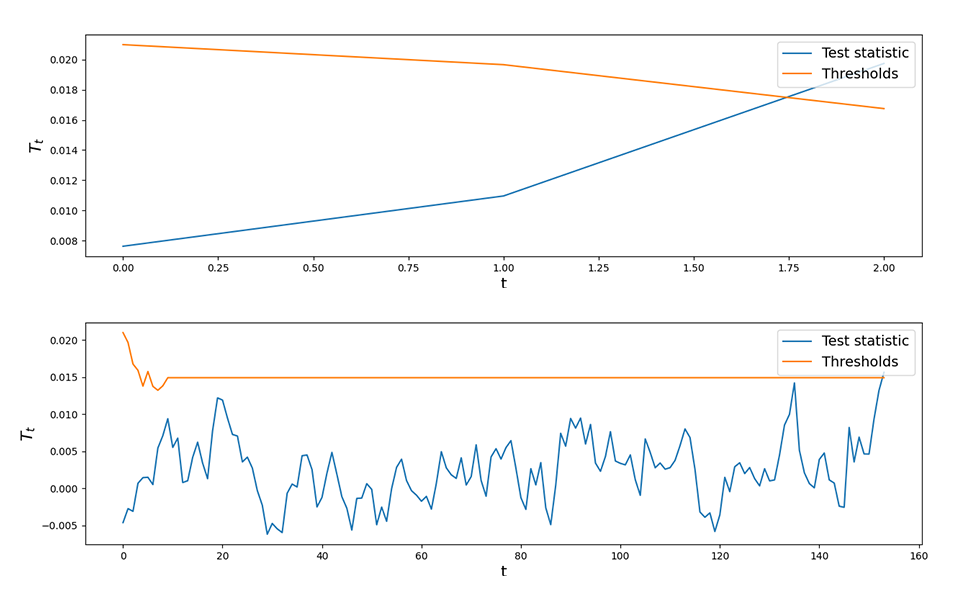
\includegraphics[width=0.6\linewidth]{bilder/drift-detection/online.png}
		\caption{Expected runtime (ERT) for corrupted and in-distribution data}\label{fig:online-ert}
	\end{center}
\end{figure}

Having such a detector one measures ERTs for not corrupted inputs, then for corrupted ones and afterwards calculates the best threshold that can separate the two. ERTs of corrupted data should be much lower than ERTs of not corrupted one. In this experiment ERTs of both classes were separable, however both located very close to the threshold: $\approx 4.59$ for corrupted ones and $\approx 7.1$ for not corrupted. Yet with a threshold of $6$ the accuracy scores are very high. Having a drift detector trained on not corrupted training data only, one can estimate ROC-AUC scores between two classes: not corrupted test data and the same test data but with some corruption applies to it. The results of this experiment with a defocus blur corruption of several severities are presented in Figure \ref{fig:online-auc-roc}. Already on severity 3, such detector separates the two almost perfectly. The scores are also presented in Table \ref{tab:severity-separability}.

\begin{figure}[htb]
	\begin{center}
		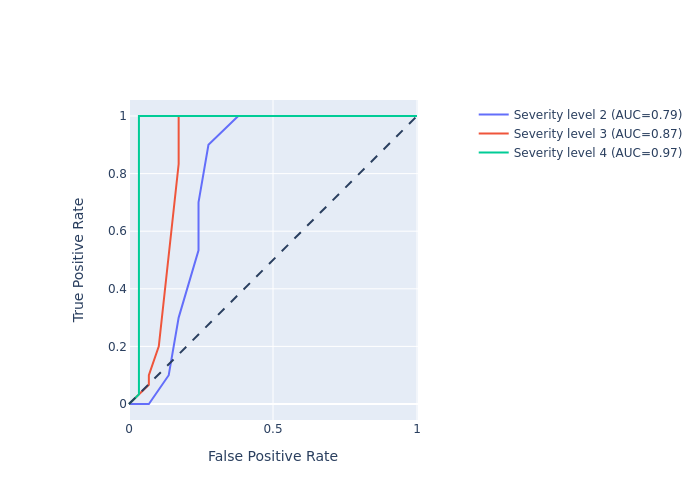
\includegraphics[width=0.8\linewidth]{bilder/drift-detection/auc_roc comparison online.png}
		\caption{AUC ROC scores for various defocus corruption severities}\label{fig:online-auc-roc}
	\end{center}
\end{figure}

\begin{table}[htb]
    \centering
    \caption{Severity of corruptions on separability}
        \begin{adjustbox}{width=0.4\textwidth}
            \begin{tabular}{|l||*{3}{c|}}\hline
                \makebox{W}
                &\makebox[3em]{Level 2}
                &\makebox[3em]{Level 3}
                &\makebox[3em]{Level 4}
                \\\hline\hline
                Auc-Roc &0.84&0.92&0.98\\\hline
            \end{tabular}
            \label{tab:severity-separability}
        \end{adjustbox}
\end{table}

Additionally, research has been performed on the influence of the hyperparameters to an online MMD drift detector, specifically: test window size, specified ERT. The results are presented in Tables \ref{tab:test-window-size-influence}, \ref{tab:ert-influence}. Test window size influences how fast and how sensitive the reaction of an algorithm should be and the ideal value in this case would be $10$ crops, during this time a threshold will be established. In case of ERT as a hyperparameter as long as it is big enough the score does not change very much.

\begin{table}[H]
    \centering
    \caption{Test window size influence on separability}
        \begin{adjustbox}{width=0.6\textwidth}
            \begin{tabular}{|l||*{5}{c|}}\hline
                \makebox{W}
                &\makebox[3em]{2}
                &\makebox[3em]{5}
                &\makebox[3em]{10}
                &\makebox[3em]{15}
                &\makebox[3em]{20}
                \\\hline\hline
                Auc-Roc &0.85&0.92&0.98&0.90&0.88\\\hline
            \end{tabular}
            \label{tab:test-window-size-influence}
        \end{adjustbox}
\end{table}

\begin{table}[H]
    \centering
    \caption{ERT influence on separability}
        \begin{adjustbox}{width=0.5\textwidth}
            \begin{tabular}{|l||*{4}{c|}}\hline
                \makebox{W}
                &\makebox[3em]{32}
                &\makebox[3em]{64}
                &\makebox[3em]{128}
                &\makebox[3em]{256}
                \\\hline\hline
                Auc-Roc &0.90&0.95&0.98&0.98\\\hline
            \end{tabular}
            \label{tab:ert-influence}
        \end{adjustbox}
\end{table}

            \paragraph{Not fixed cells imaging as corrupted input}
                In section \ref{section:gfp} the difference between fixed and not fixed cells was mentioned. Visual analysis of model's predictions for not fixed cells after training it on fixed ones has shown that the model was not able to generalize well on them. That is why it would be important to alarm the end-user to not rely on predictions when such situation occurs. In this case an online drift detector trained using not corrupted data used for ER training first and tested on not fixed ER cells. The results of this test are shown in Figure \ref{fig:online-drift-not-fixed}.
                \begin{figure}[H]
                    \begin{center}
                        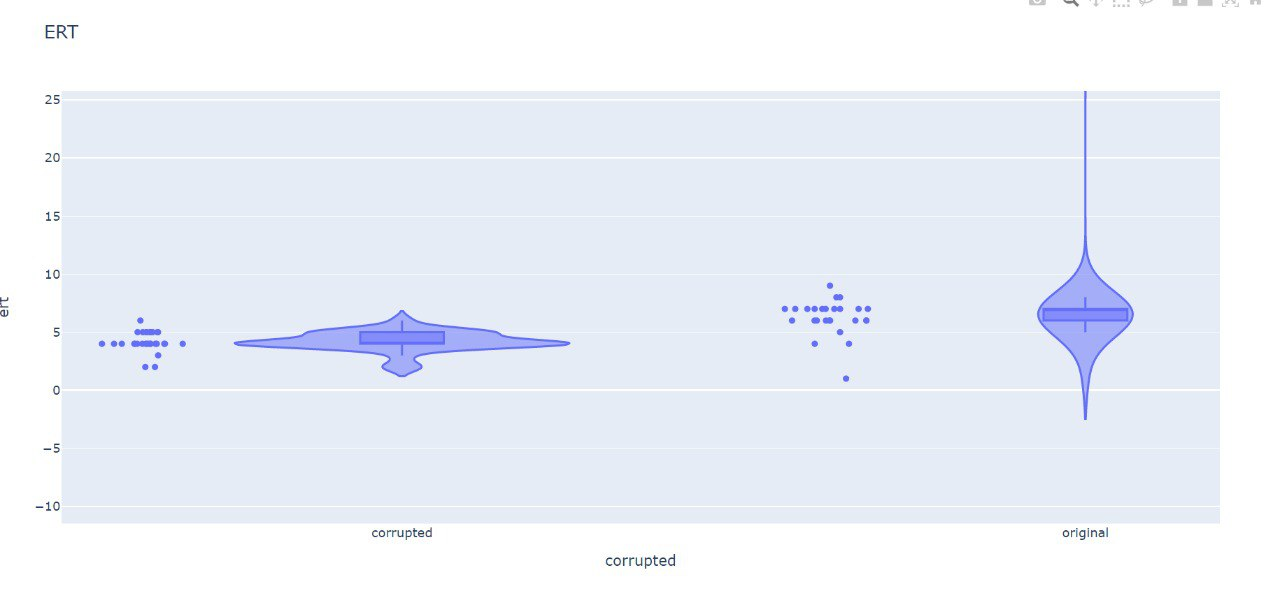
\includegraphics[width=0.5\linewidth]{bilder/drift-detection/online-fixed-vs-not-fixed.jpg}
                        \caption{Online drift detection of not fixated cells}\label{fig:online-drift-not-fixed}
                    \end{center}
                \end{figure}
                The ERTs for corrupted data (left) are lower from ERT for true input. ROC-AUC score for the separability is $0.91$ and the best threshold is $6$. However not corrupted data (fixed cells) mostly have ert of $7$, whereas corrupted data (not fixed cells) have an ert of $4$. Both classes have ERTs that are very close to the threshold.